% 
% Licensed to the Apache Software Foundation (ASF) under one
% or more contributor license agreements.  See the NOTICE file
% distributed with this work for additional information
% regarding copyright ownership.  The ASF licenses this file
% to you under the Apache License, Version 2.0 (the
% "License"); you may not use this file except in compliance
% with the License.  You may obtain a copy of the License at
% 
%   http://www.apache.org/licenses/LICENSE-2.0
% 
% Unless required by applicable law or agreed to in writing,
% software distributed under the License is distributed on an
% "AS IS" BASIS, WITHOUT WARRANTIES OR CONDITIONS OF ANY
% KIND, either express or implied.  See the License for the
% specific language governing permissions and limitations
% under the License.
% 
% Create well-known link to this spot for HTML version
\ifpdf
\else
\HCode{<a name='DUCC_WEBSERVER'></a>}
\fi
\chapter{DUCC Web Server}

    The {\DUCC} Web Server default address is accessed from the URL http://[DUCC-HOST]:42133.  The
    {\em[DUCC-HOST]} is the hostname where the local installation has installed the {\DUCC}
    Web Server.
    
  \begin{center}     
  \cfbox{green}{The hostname and port are configurable by
  the {\DUCC} administrator in ducc.properties}
  \end{center}
  
    The Webserver is designed to be mostly self-documenting. The design is intentionally simple 
    and contains a link to this document.  Most of the interesting fields and column headers
    have ``mouse hovers'' which display a short 
    description if you hover your mouse pointer over it for a moment.

\begin{figure}[ht!]
\centering
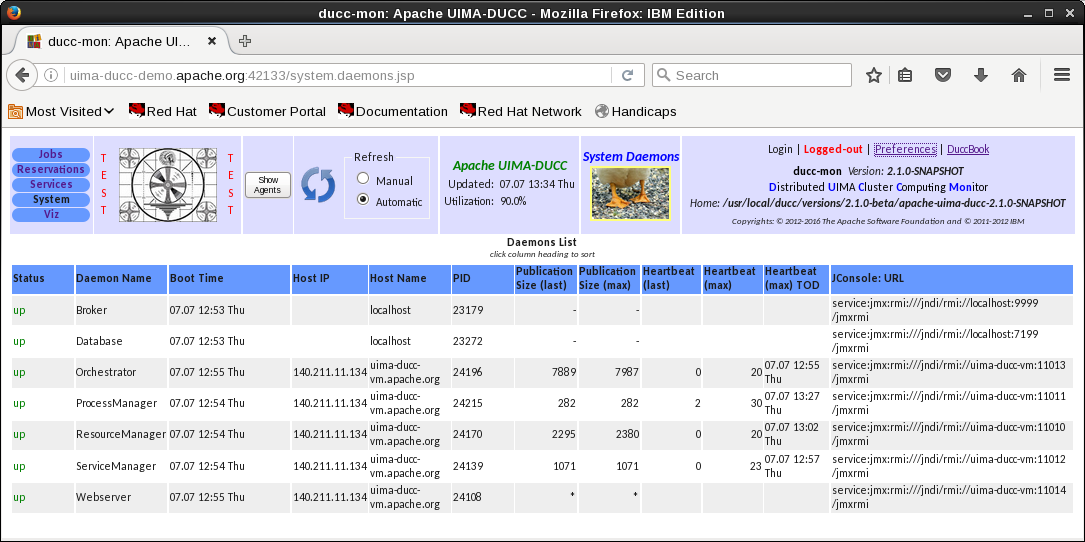
\includegraphics[width=90mm]{images/ducc-webserver/System-Daemons.png}
\caption{Sample Webserver Page}
\end{figure}

    Normally, the Web Server automatically fetches new data from {\DUCC} and updates the display.
    This is controlled by setting one of the two refresh modes:
    \begin{itemize}
      \item Manual refresh.  In this mode, the browser windows are updated only by using the
        browser's refresh button, or the {\DUCC} refresh button to the left in the header of
        each page.
      \item Automatic refresh. In this mode, the browser automatically fetches and displays
        new data.  The rate of refresh is currently fixed and cannot be configured.
    \end{itemize}
    
    There is a behavior difference between refresh and reload.
    \paragraph{Refresh}
    Refresh causes the current data on the page to be updated with the most
    current information in the Webserver's possession.  This is performed
    when the refresh button is clicked.
    \paragraph{Reload}
    Reload occurs when the enter key is pressed.  Reload causes not just the
    data to be updated but rather the entire page is replaced.
    
    Two different table styles are supported:
    \begin{itemize}
      \item Scroll, and
      \item Classic.
    \end{itemize}
    Table styles are switched using the {\em Preferences} link.

    \paragraph{Scroll Mode}  When {\em scroll table style} is the preference, a scroll bar is
    shown to the right, within the main window.  The scroll bar allows scrolling to be restricted to the data
    display, leaving column and {\DUCC} headers in place.  In this mode any column may be sorted
    simply by clicking on it.
    
    With respect to sorting, any specified sort is remembered for refresh
    but forgotten for reload.  Sorting is permitted when either manual
    or automatic refresh mode is selected.
    
    The column sort order is maintained until the page is reloaded.

	Note that not all pages have a scroll version - some only have a classic version.
	
    \paragraph{Classic Mode}  When {\em classic table style} is the preference, the
    main data may extend below the bottom of the page and it will be necessary to use the browser's scroller on the right
    to access it.  The column headers and {\DUCC} header scrolls off when doing this.  Columns
    may be sorted in this mode but it is necessary to first switch to ``Manual'' refresh mode to
    prevent browser refreshes during sorting and display of data. 
    
    With respect to sorting, any specified sort is forgotten for refresh
    and reload.  Sorting is only permitted when manual refresh mode is
    selected.
    
    The column sort order is maintained until the page is refreshed or reloaded.

\begin{figure}[ht!]
\centering
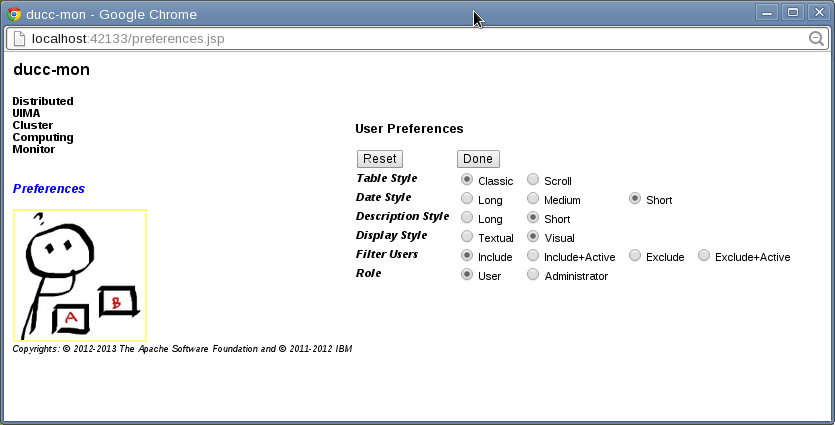
\includegraphics[width=90mm]{images/ducc-webserver/Preferences.png}
\caption{Preferences Page}
\end{figure}

% Create well-known link to this spot for HTML version
\ifpdf
\else
\HCode{<a name='DUCC_WS_COMMON'></a>}
\fi
    \section{Common Links}

        Every page contains a common header containing links and controls. The links permit navigation
        to other content at the site. The controls provide page-wise configuration of the content at
        that page.

        The following links are available on every page of the web server: 

        \begin{description}
          \item[Authentication] \hfill \\ 
            Authentication is needed in order to cancel jobs and reservations, to create a
            reservation, and to perform administration. It is not required to simply view the pages.

            \begin{itemize}
              \item Login - Authenticate and start a session with the Web Server.             
              \item Logout - Terminate the Web Server session 
            \end{itemize}

          \item[Preferences]
            The following preferences may be set:
            \begin{description}
              \item[Table Style] This selects ``scroll'' or ``classic'' display, as
                described above.
              \item[Date Style] This selects long, medium, or long formats for dates.
              \item[Description Style] This selects long or short formats for the various
                description fields.
              \item[Display Style] Choose to display text or (in some circumstances) icons.
              \item[Filter Users] This controls the ``filter'' box near the middle of
                the header on each page.  It allows various levels of inclusion and
                exclusion of active or completed work for the filtered users.
              \item[Role] This allows selection of ``User'' or ``Administrator'' roles.
                This protects registered {\DUCC} administrators from accidentally affecting
                other people's work.
            \end{description}
            
          \item[DuccBook] \hfill \\
            This is a link to the HTML version of the document you are reading.

          \item[Jobs] \hfill \\
            This navigates to the Jobs page, showing all the jobs in the system.

          \item[Reservations] \hfill \\
            This navigates to the Reservations page, showing all the reservations
            in the system and provides a button that can be used to request new reservations. 

          \item[Services] \hfill \\
            This navigates to the Services page, showing all the services in the
            system.

          \item[System] \hfill \\
            This opens a sub-menu with system-related links:
            \begin{itemize}
              \item Administration - This opens a page with administrative functions. 
              \item Broker - This shows information about the AMQ broker employed by the system. 
              \item Classes - This shows all the scheduling classes defined to the system. 
              \item Daemons - This shows the status of {\DUCC}'s management processes. 
              \item DuccBook - This manual. 
              \item Machines - This shows the status of all the {\DUCC} worker nodes. 
            \end{itemize}

            \item[Viz]
            This opens a page with a visualization of the system hosts, showing all
            scheduled work in the system.
      \end{description}              

      % Create well-known link to this spot for HTML version
      \ifpdf
      \else
      \HCode{<a name='DUCC_WS_JOBS'></a>}
      \fi
      % 
% Licensed to the Apache Software Foundation (ASF) under one
% or more contributor license agreements.  See the NOTICE file
% distributed with this work for additional information
% regarding copyright ownership.  The ASF licenses this file
% to you under the Apache License, Version 2.0 (the
% "License"); you may not use this file except in compliance
% with the License.  You may obtain a copy of the License at
% 
%   http://www.apache.org/licenses/LICENSE-2.0
% 
% Unless required by applicable law or agreed to in writing,
% software distributed under the License is distributed on an
% "AS IS" BASIS, WITHOUT WARRANTIES OR CONDITIONS OF ANY
% KIND, either express or implied.  See the License for the
% specific language governing permissions and limitations
% under the License.
% 

    \section{Jobs Page}
    \label{sec:ws.jobs-page}
        The Web Server's home page is also the Jobs page. This page has links to all the rest of the content 
        at the site and shows the status of all the jobs in the system. 
    
        The Jobs page contains the following columns: 

        \begin{description}

            \item[Id] \hfill \\
              This is the ID as assigned by {\DUCC}. This field is hyperlinked to a
              \hyperref[sec:ws-job-details]{Job Details} page for that job that shows the breakdown of
              all the processes assigned to the job and their state.
              
            \item[Start] \hfill \\
              This is the time the Job is accepted into {\DUCC}.
              
            \item[Duration] \hfill \\
              This shows two times.  In green the length of time the job has been running.  In black is
              the estimated time of completion, based on current resources and remaining work.  When
              the job completes, the time shown is the total elapsed time of the job.
                            
            \item[User] \hfill \\
              This is the userid of the job owner.
              
            \item[Class] \hfill \\
              This is the resource class the job is submitted to.
              
            \item[State] \hfill \\
              This shows the state of the job.  The normal job progression is shown below, with an
              explanation of what each state means.
              \begin{description}
                  \item[Received] - The job has been vetted, persisted, and assigned a unique ID. 
                  \item[WaitingForDriver] - The job is waiting for the Job Driver to initialize. 
                  \item[WaitingForServices] - The job is waiting for verification from the
                    Service Manager that required services are started and responding.  This may
                    cause {\DUCC} to start services if necessary.  In that even this state will
                    persist until all pre-requisite services are ready.
                  \item[WaitingForResources] - The job is waiting to be scheduled. In busy
                    systems this may require preemption of existing work.  In that case this
                    state will persist until preemption is complete.
                  \item[Initializing] - The job initializing. Usually this
                    is the UIMA-AS initialization phase.  In the default configuration, only
                    two (2) processes are allocated by the Resource Manager.  No additional
                    resources are allocated until at least one of the new processes successfully
                    completes initialization.  Once initialization is complete the Resource Manager
                    will double the number of allocated processes until the user's fair share of
                    the resources is attained.
                  \item[Running] - At least one process is now initialized and running. 
                  \item[Completing] - The last work item has completed and {\DUCC} is freeing resources.
                    If the job had many resources allocated at the time the job exited this state
                    will persist until all allocated resources are freed.
                  \item[Completed] - The job is complete. 
              \end{description}
                  
            \item[Reason or Extraordinary Status] \hfill \\

              % See this structure:
              % org.apache.uima.ducc.transport.event.common.IDuccCompletionType
              
              This field contains miscellaneous information pertaining to the job.  If the job exits
              the system for any reason, that reason is shown here.  If the job's pre-requisite
              services are unavailable (or ailing) that fact is displayed here.  If there is a
              job monitor running, that fact is shown here.  Most of the values for this field
              support ``hovers'' containing additional information about the reason.
         
              \begin{description}
                  \item[EndOfJob] - The job and completed ran with no errors. 
                  \item[Error] - All work items are processes but at least one had an error. 
                  \item[CanceledByDriver] - The Job Driver (JD) terminated the job. The reason for
                    termination is seen by hovering over the text with your mouse.
                  \item[CanceledBySystem] - The job was canceled because {\DUCC} was shutdown. 
                  \item[CanceledBySser] - The job owner or {\DUCC} administrator canceled the job. 
                  \item[Cancel Pending] - The job has been canceled and is not yet fully evicted
                    from the system.
                  \item[DriverInitializationFailure] - The Job Driver (JD) process is unable to initialize. Hover over 
                    the field with your mouse for details (if any are available), and check your JD log. 
                  \item[DriverProcessFailed] - The Job Driver (JD) process failed for some reason. Hover over the 
                    field with your mouse for details (if any), and check your JD log. 
                  \item[MonitorActive] The job has a console monitor active.  This is enabled with the
                    job's ``wait\_for\_completion'' parameter on job submission.
                  \item[ServicesUnavailable] - The job declared a dependency on one or more services, and the 
                    Service Manager (SM) cannot find or start the required service. 
                  \item[Premature] - The job was terminated for some unknown reason before all work items were 
                    processed. Check the JP logs for details. 
                  \item[ProcessInitializationFailure] - Too many processes failed during
                    initialization and the job was canceled by {\DUCC}.  Check the JP logs for the
                    reason.
                  \item[ProcessFailure] - Too many processes failed while running and {\DUCC} canceled
                    the job.  Check the JP logs for the reason.
                  \item[ResourcesUnavailable] - The Resource Manager (RM) is unable to allocate resources for 
                    the job. For non-preemptable jobs this could be because the limit on that type of allocation is 
                    reached, or all the hosts are already allocated and work cannot be preempted to make space for 
                    it. For all jobs, it could be because the job class is invalid. 
                    \item[{\em service\_name}] If there is a service name in this field it indicates the job is
                      dependent on the service but the service is not responding to the {\DUCC} Service Monitor's
                      pinger.
              \end{description}

            \item[Services] \hfill \\
              This is the number of services the job has declared dependencies on.  There is a ``hover'' that
              shows the ids of the services, if any.

            \item[Processes] \hfill \\
              This is the number of processes currently assigned to the job.

            \item[Init Fails] \hfill \\
              This is the total number of initialization failures experienced by the job. This
              field is hyperlinked to pages with log excerpts highlighting the specific failures.
              
            \item[Run Fails] \hfill \\
              This is the total number of process failures experienced by the job. This field is
              hyperlinked to pages with log excerpts highlighting the specific failures.
              
            \item[PgIn] This is the number of page-in events, over all processes, on the machines
              running the job.

            \item[Swap] This is the total swap space, over all the processes, being used by the job.

            \item[Size] \hfill \\
              This is the declared memory size of the job
              
            \item[Total] \hfill \\
              This is the total number of work items declared by the job.
              
            \item[Done] \hfill \\
              This is the total number of work items successfully completed for the job.
              
            \item[Error] \hfill \\
              This is the total number of exceptions thrown or other errors experienced by work
              items. This field is hyperlinked to pages containing log excerpts highlighting
              the failures.
              
            \item[Dispatch] \hfill \\
              This is the total number CASs that are currently dispatched. 

              This usually represents the quantity derived from the following formula:
\begin{verbatim}              
     min( (initialized.processes * threads.per.process), (incomplete.work.items - errors) )
\end{verbatim}

              The actual number is a measured number, not a calculated number, and may differ
              slightly from the formula if the measurement is taken immediately after process
              start-up, or in the time between a work item completing and a new one being
              dispatched.
              
            \item[Retry] \hfill \\
              This is the number of CASs that were retried for any reason.  Reasons for retry
              include preemption for fair-share, work-item timeout, or error conditions.

              Note: If a work item in any process fails, the entire process is considered
              suspect, and all work-items in the process are terminated.  Work items in the
              process which did not have errors are re-dispatched (retried) to a different
              process.
              
            \item[Preempt] \hfill \\
              This is the total number of processes that have been preempted to make room for
              other work due to Fair Share.
              
            \item[Description] \hfill \\
              This is the description string from the $--$description string from submit.
            \end{description}

    \begin{figure}[ht!]
    \centering
    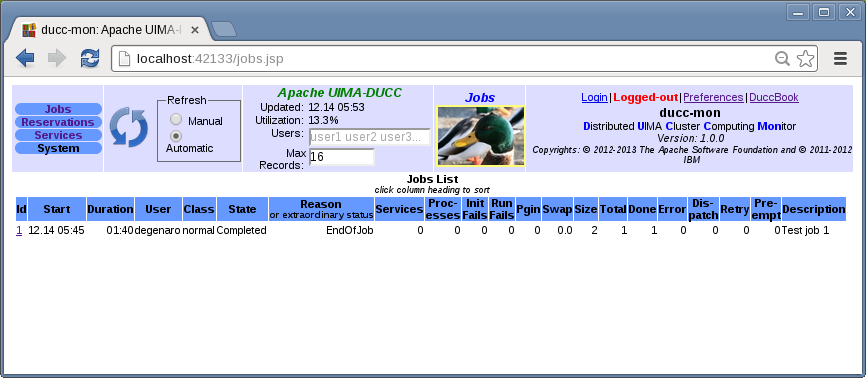
\includegraphics[width=90mm]{images/ducc-webserver/Jobs.png}
    \caption{Jobs Page}
    \end{figure}
            


      % Create well-known link to this spot for HTML version
      \ifpdf
      \else
      \HCode{<a name='DUCC_WS_JOB_DETAILS'></a>}
      \fi
      % 
% Licensed to the Apache Software Foundation (ASF) under one
% or more contributor license agreements.  See the NOTICE file
% distributed with this work for additional information
% regarding copyright ownership.  The ASF licenses this file
% to you under the Apache License, Version 2.0 (the
% "License"); you may not use this file except in compliance
% with the License.  You may obtain a copy of the License at
% 
%   http://www.apache.org/licenses/LICENSE-2.0
% 
% Unless required by applicable law or agreed to in writing,
% software distributed under the License is distributed on an
% "AS IS" BASIS, WITHOUT WARRANTIES OR CONDITIONS OF ANY
% KIND, either express or implied.  See the License for the
% specific language governing permissions and limitations
% under the License.
% 
  
    \section{Job Details Page}
    \label{sec:ws-job-details}

    This page shows details of all the processes that run in support of a job. 
    The information is divided among five tabs:
    \begin{description}
      \item[Processes] This tab contains details on all the processes for the job, both
        active, and defunct.
      \item[Work Items] This tab shows details for each individual work-item in the job.
      \item[Performance] This tab shows a performance break-down of all the UIMA analytics
        in the job.
      \item[Specification] This tab shows the job specification for the job.
      \item[Files] This tab shows the files in the log directory.
      \end{description}
      
    \subsection{Processes}
    \label{subsec:ws-processes}
    The processes page contains the following columns:
    
    \begin{description}

        \item[Id] \hfill \\
          This is the {\DUCC}-assigned numeric id of the process (not the Operating System's
          process Id). Process 0 is always the Job Driver.          

        \item[Log] \hfill \\
          This is the log name for the process. It is hyperlinked to the log itself.

        \item[Log Size] \hfill \\
          This is the size of the log in MB. If you find you have trouble viewing the log
          from the Web Server it could be because it is too big to view in the server and needs to
          be read by some other means than the Web Server.  (It is not currently paged in by 
          the Web Server, it is read in full.)

        \item[Host Name] \hfill \\
          This is the name of the host where the process ran.

        \item[PID] \hfill \\
          This is the Unix process ID (PID) of the process.

        \item[State Scheduler] \hfill \\
          % The information comes from here:
          % State Scheduler: org.apache.uima.ducc.transport.event.common.IResourceState.ResourceState

          This shows the Resource Manager state of the job. It is one of:
          \begin{description}
              \item[Allocated] - The host is currently allocated for this job by the RM.
              \item[Deallocated] - The resource manager has deallocated the shares for the job on
                this host.
          \end{description}

        \item[Reason Scheduler or extraordinary status] \hfill \\
          \phantomsection\label{itm:job-details-sched}


          % The information comes from here:
          % Reason Scheduler: org.apache.uima.ducc.transport.event.common.IResourceState.ProcessDeallocationType
          This column provides a reason for the scheduler state, when the scheduler state is other than ``Allocated''. 
          These may have ``hovers'' that provide more information
          if it is available.

            \begin{description}          
                \item[AutonomousStop] - The process terminated unexpectedly of its own accord ("crashed", or
                  simply exited.) 

                \item[Exception] - The process is terminated by the JD exception handler. 

                \item[Failed] - The process is terminated by the Agent because the JP wrapper was able to detect and 
                  communicate a fatal condition (Exception) in the pipeline.. 
                  
                \item[FailedInitialization] - The process is terminated because the UIMA initialization step failed. 
                  
                \item[Forced] - The host is preempted by RM for other work because of fair share. 
                  
                \item[JobCanceled] - The job was canceled by the user or a system administrator. 
                  
                \item[JobCompleted] - The process is canceled because of {\DUCC} restart. 
                  
                \item[JobFailure] - The job failure limit is exceeded, causing the job to be canceled by the JD.                    
                  
                \item[InitializationTimeout] - The UIMA initialization phase exceeded the configured timeout. 
                  
                \item[Killed] - The agent terminated the process for some reason. The ``Reason Agent'' field
                  should have more details in this case.
          
                \item[Stopped]	- The process was terminated by the Agent for some reason.  The hover should
                  contain more information.
                          
                \item[Voluntary] - The job is winding down, there's no more work for this host, so it stops. 
                  
                \item[Unknown] - None of the above. This is an exceptional condition, sometimes an
                  internal {\DUCC} error. Check the JP and JD logs for possible causes..
            \end{description}

          \item[State Agent] \hfill \\
          \phantomsection\label{itm:job-details-state}

          % This state comes from here:
          % State Agent: org.apache.uima.ducc.transport.event.common.IProcessState.ProcessState
            This shows the {\DUCC} Agent's view of the state of the process.
            \begin{description}
               \item[Starting] The {\DUCC} process manager as issued a request to the assigned {\DUCC} Agent to
                 start the process.
               \item[Initializing] The process is initializing.  Usually this means the UIMA analytic
                 pipeline (Job Process) is executing its initialization method.
              \item[Running] The Job Process has completed the initialization phase and is ready for 
                or actively executing work.
              \item[Stopped] The {\DUCC} Agent reports the process is stopped and (and has exited).
              \item[Failed] The {\DUCC} Agent reports the process failed with errors.  This usually
                means that UIMA-AS has detected exceptions in the pipeline and reported them
                to the Job Driver for logging.
              \item[FailedInitialization] The process died during the UIMA initialization phase.
              \item[InitializationTimeout] The process exceeded the site's limit for time spent
                in UIMA initialization.
              \item[Killed] The {\DUCC} Agent killed the process for some reason.  There are
                three reasons for this:
                \begin{enumerate}
                  \item The Job Processes failed to initialize,
                  \item The Job Process timed out during initialization,
                  \item The process exceeded its allowed swap.
                \end{enumerate}
              \item[Abandoned] It is possible to cancel a specific process of a job.  Usually
                this is because it became ``stuck'' because of hardware failure.  If a process
                is killed in \hyperref[sec:cli.ducc-cancel]{this way}, the state is recorded as {\em Abandoned}.
            \end{description}
            
          \item[Reason Agent] \hfill \\
          \phantomsection\label{itm:job-details-agent}

          This shows extended reason information if a process exited other than having run out
          of work to do.

            \begin{description}
              \item[AgentTimedOutWatingForORState] The {\DUCC} Agent is expecting a state update
                from the {\DUCC} Orchestrator.  Timer on this wait has expired.  This usually 
                indicates an infrastructure or communication problem.
              \item[Croaked] The process exited for no good or clear reason, it simply vanished.
              \item[Discontinued] This is the normal reason when the process is stopped as directed.
              \item[ExceededShareSize] The process exceeded it's declared memory size.
              \item[ExceededSwapThreshold] The process exceeded the configured swap threshold.
              \item[FailedInitialization] The process was terminated because the UIMA 
                initialization step failed.
              \item[InitializationTimeout] The process was terminated because the UIMA initialization
                step took too long.
              \item[JPHasNoActiveJob] This is set when an agent looses connectivity while its
                JPs are running. The job finishes (stopped or killed). The agent regains
                connectivity. The OR publish no longer includes the job but the agent still has
                processes running for that job. The agent kills ghost processes with the reason:
                JPHasNoActiveJob.
              \item[LowSwapSpace] The process was terminated because the system is about to run
                out of swap space.  This is a preemptive measure taken by {\DUCC} to avoid exhaustion
                of swap, to effect orderly eviction of the job before the operating system starts
                its own reaping procedures.
              \item[AdministratorInitiated] The process was canceled by an administrator.
              \item[UserInitated] The process was canceled by the owning user.
            \end{description}
                    
          \item[Exit] \hfill \\
            The process exit code or signal.
            
          \item[Time Init] \hfill \\
            This is the clock time this process spent in initialization.
            
          \item[Time Run] \hfill \\
            This is the clock time this process spent in executing, not including
            initialization.
            
          \item[Time GC] \hfill \\
            This is amount of time spent in Java Garbage Collection for the process.
            
          \item[PgIn] \hfill \\
            This is the number of page-in events on behalf of the process.

          \item[Swap] \hfill \\
            This is the amount of swap space on the machine being consumed by the process.

          \item[\%CPU] \hfill \\
            Current CPU percent consumed by the process.  This will be $>$ 100\% on 
            multi-core systems if more than one core is being used.  Each core contributes
            up to 100\% CPU, so, for example, on a 16-core machine, this can be as high
            as 1600\%.
            
          \item[RSS] \hfill \\
            The amount of real memory being consumed by the process (Resident Storage Size)
            
          \item[Time Avg] \hfill \\
            This is the average time in seconds spent per work item in the process.
            
          \item[Time Max] \hfill \\
            This is the maximum time in seconds spent per work item in the process.
            
          \item[Time Min] \hfill \\
            This is the minimum time in seconds spent per work item in the process.
            
          \item[Done] \hfill \\
            This is the number of work items processed in this process.
            
          \item[Error] \hfill \\
            This is the number of exceptions processing work items in this process.
                      
          \item[Dispatch] \hfill \\
            The number of work items currently dispatched.
              
          \item[Retry] \hfill \\
            This is the number of work items that were retried in this process for any reason, excluding
            preemption.
            
          \item[Preempt] \hfill \\
            This is the number of work items that were preempted from this process, if
            fair-share caused preemption.
            
          \item[JConsole URL] \hfill \\
            This is a URL that can be used to connect via JMX to the processes, e.g. via
            jconsole.

      \end{description}
      
    \begin{figure}[ht!]
    \centering
    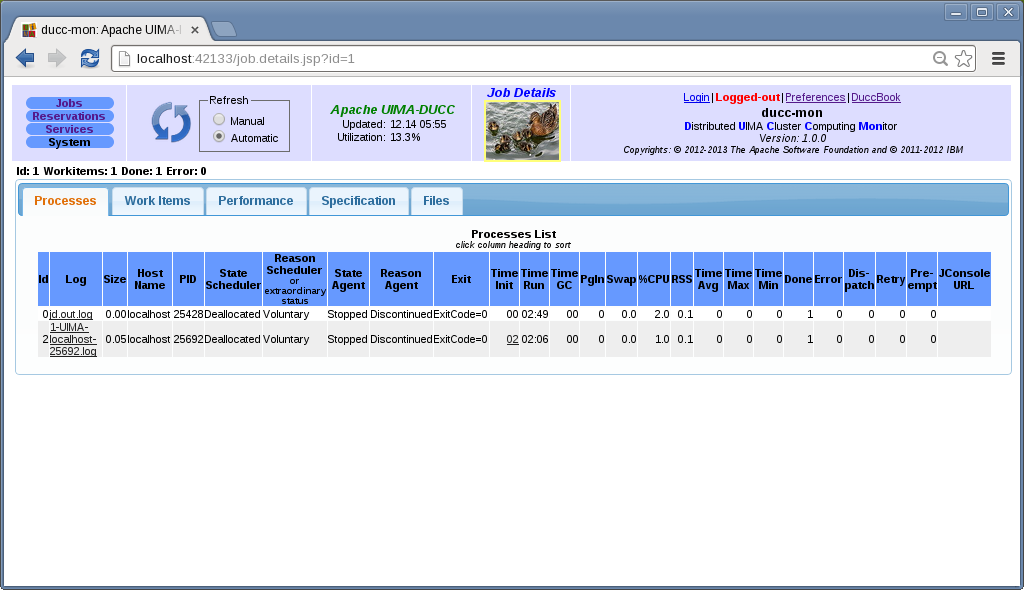
\includegraphics[width=90mm]{images/ducc-webserver/Job-Details-Processes.png}
    \caption{Processes Tab}
    \end{figure}
    
   \subsection{Work Items}
   \label{subsec:ws-work-items}
   This tab provides details for each individual work item.  Columns include:

   % The data comes from here: org.apache.uima.ducc.common.jd.files.IWorkItemState.State    
   \begin{description}
     \item[SeqNo]  \hfill \\
       This is the sequence work items are fetched from the Collection Reader's
       getNext() method by the {\DUCC} Job Driver.
     \item[Id]  \hfill \\
       This is the name of the work item.
     \item[Status]  \hfill \\
       The is the current state of the work item.  
       States include:
       \begin{description}
         \item[ended] The work item is complete.
         \item[error] The work item ended with errors.
         \item[operating] The work item is current being executed.
         \item[retry] The work item is being retried.
         \item[start] The work item has been picked up for execution and {\DUCC} is waiting
           for confirmation that it is running.
       \end{description}
       If a work item has not yet been retrieved from the Collect Reader it does not show
       on this page.
     \item[Delivery Time (sec)]  \hfill \\
       The time spent in getting a work item from the Job Driver to a Job Process.
     \item[Process Time (sec)]  \hfill \\
       The time spent processing the work item.
     \item[Investment Time (sec)]  \hfill \\
       The time spent processing the work item during the current epoch.
     \item[Node (IP)]  \hfill \\
       The host IP where the work item was processed.
     \item[Node (Name)]  \hfill \\
       The host name where the work item was processed.
     \item[PID]  \hfill \\
       The Unix Process Id that the work item was processed in.
   \end{description}
    
    \begin{figure}[ht!]
    \centering
    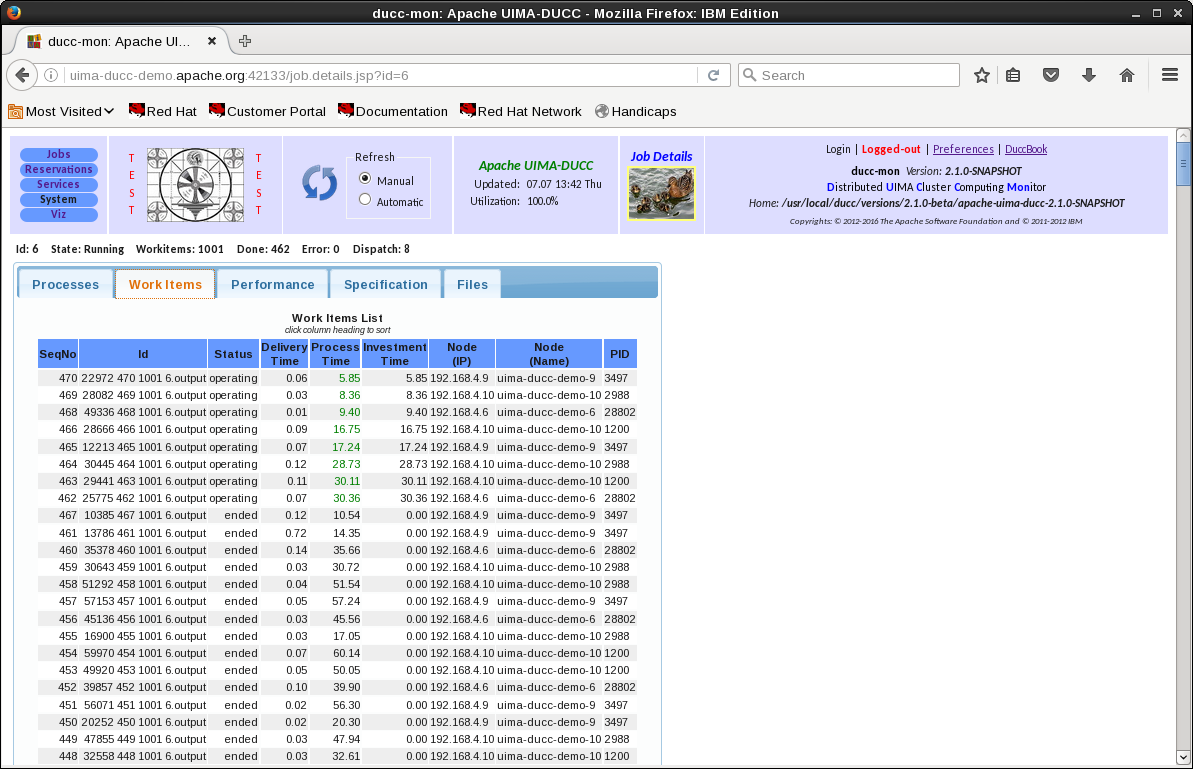
\includegraphics[width=90mm]{images/ducc-webserver/Job-Details-WorkItems.png}
    \caption{Work Items Tab}
    \end{figure}  

   \subsection{Performance}
   \label{subsec:performance}
   This tab shows performance summaries of all the pipeline components.  The statistics
   are aggregated over all instances of each component in each process of the job.
   
   \begin{description}
     \item[Name]  \hfill \\
       The short name of the analytic.
     \item[Total]  \hfill \\
       This is the total time in days, hours, minutes, and seconds taken by each
       component of the pipeline.
     \item[\% of Total]  \hfill \\
       This is the percent of the total usage consumed by this analytic.
     \item[Avg]  \hfill \\
       This is the average time spent by all the instances of the analytic.
     \item[Min]  \hfill \\
       This is the minimum time spent by any instance of the analytic.
     \item[Max]  \hfill \\
       This is the maximum time spent by any instance of the analytic.
   \end{description}
    
    \begin{figure}[ht!]
    \centering
    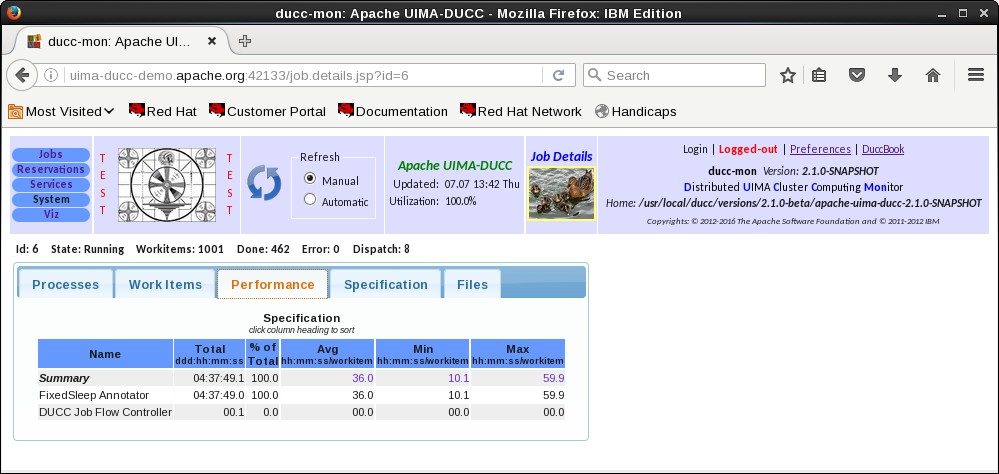
\includegraphics[width=90mm]{images/ducc-webserver/Job-Details-Performance.png}
    \caption{Performance Tab}
    \end{figure}  
       
   \subsection{Specification}
   This tab shows the full job specification in the form of a Java Properties
   file.  This will include all the parameters specified by the user, plus those
   filled in by {\DUCC}.
    
    \begin{figure}[ht!]
    \centering
    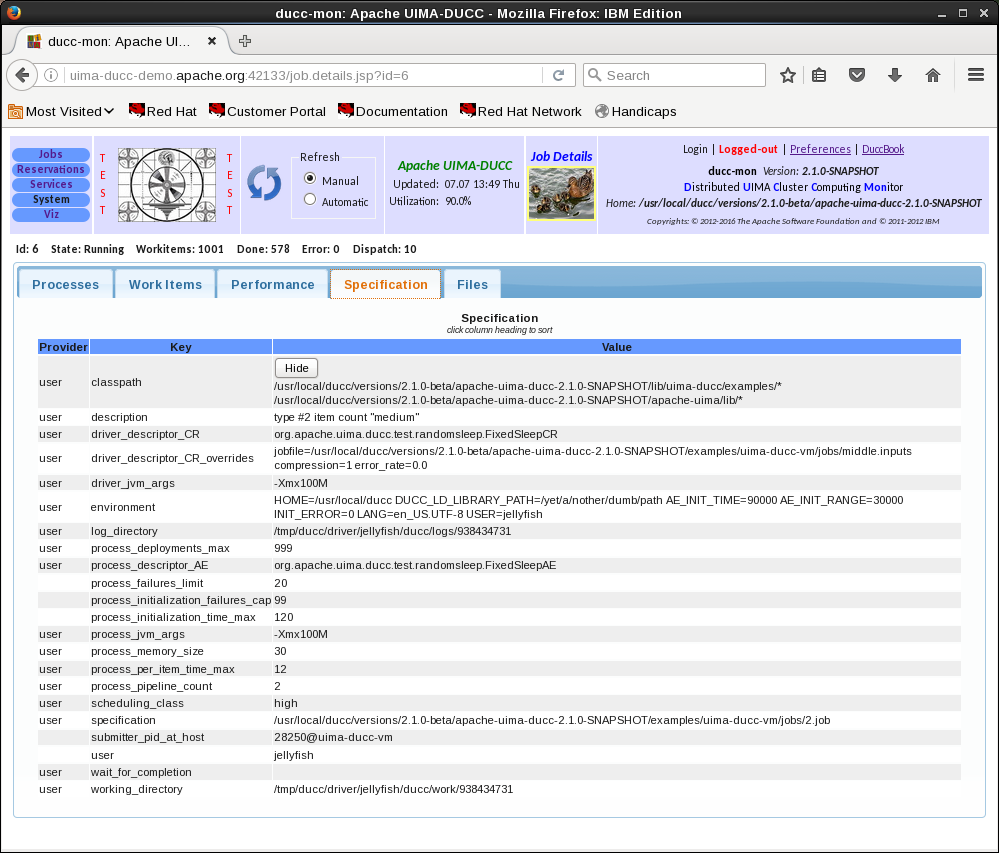
\includegraphics[width=90mm]{images/ducc-webserver/Job-Details-Specification.png}
    \caption{Specification Tab}
    \end{figure}  
    
   \subsection{Files}
   This tab shows the files in the log directory.


      % Create well-known link to this spot for HTML version
      \ifpdf
      \else
      \HCode{<a name='DUCC_WS_RESERVATIONS'></a>}
      \fi
      % 
% Licensed to the Apache Software Foundation (ASF) under one
% or more contributor license agreements.  See the NOTICE file
% distributed with this work for additional information
% regarding copyright ownership.  The ASF licenses this file
% to you under the Apache License, Version 2.0 (the
% "License"); you may not use this file except in compliance
% with the License.  You may obtain a copy of the License at
% 
%   http://www.apache.org/licenses/LICENSE-2.0
% 
% Unless required by applicable law or agreed to in writing,
% software distributed under the License is distributed on an
% "AS IS" BASIS, WITHOUT WARRANTIES OR CONDITIONS OF ANY
% KIND, either express or implied.  See the License for the
% specific language governing permissions and limitations
% under the License.
% 

\section{Reservations Page}
\label{sec:ws-reservations}

This page shows details of all reservations.  There are two types of reservations: {\em managed}
and {\em unmanaged}.

A {\em managed reservation} is a reservation whose process is fully managed by {\DUCC}.  This process
is any arbitrary process and is submitted with the
\hyperref[sec:cli.ducc-process-submit]{ducc\_process\_submit} CLI.  The lifetime of the reservation
starts at the time {\DUCC} assigns a unique ID, and ends when the process terminates for any reason.

An {\em unmanaged reservation} is essentially a sandbox for the user.  {\DUCC} starts no processes
in the reservation and manages none of the processes which run on that host.  The lifetime of the
reservation starts at the time {\DUCC} assigns a unique ID, and ends when the submitter or system
administrator cancels it.

The Reservations page contains the following columns: 
\begin{description}

\item[Id] \hfill \\
  This is the unique {\DUCC} numeric id of the reservation as assigned when the reservation is made.
  If this is a {\em managed} reservation, the ID is hyperlinked to a
  \hyperref[sec:ws-managed-reservation-details]{Managed Reservation Details} page with extended
  details on the process running in the reservation.

\item[Start] \hfill \\
  This is the time the reservation was made.
  
\item[Duration] \hfill \\
  A time in green is the length of time the active reservation has been assigned.  
  A time in black is the length of time the completed reservation was assigned. 
  
\item[User] \hfill \\
  This is the userid that made the reservation.
  
\item[Class] \hfill \\
  This is the scheduling class used to schedule the reservation.
  
\item[Type] \hfill \\
  This is the reservation type, {\em managed} or {\em unmanaged}, as described 
  \hyperref[sec:ws-reservations]{above}.

\item[State] \hfill \\
  % 1. org.apache.uima.ducc.transport.event.common.IDuccState
  This is the status of the reservation. Values include: Received - Reservation
  has been vetted, persisted, and assigned unique Id.
  \begin{description}
  \item[Assigned] - The reservation is active. 
  \item[Completed] - The reservation has been terminated.
  \item[Received] - The Reservation has been vetted, persisted, and assigned a unique ID.
  \item[WaitingForResources] - The reservation is waiting for the Resource Manager to find and 
    schedule resources. 
  \end{description}

\item[Reason] \hfill \\

  % 2. org.apache.uima.ducc.transport.event.common.IDuccCompletionType

  If a reservation is not active, this shows the reason.  Note that for
  {\em unmanaged reservations}, even if the user has processes running in the
  reservation, {\DUCC} does NOT attempt to terminate those processes (hence, ``unmanaged''.)

  For {\em managed reservations}, {\DUCC} does terminate the associated process.

  \begin{description}
  \item[CanceledBySystem] - In the case of the special JobDriver reservation, this is
    canceled by {\DUCC} and reestablished on reboot; hence the state is a result of {\DUCC}
    having been restarted.

    In all other cases, it is a result of {\DUCC} being restarted {\em COLD}.  When
    {\DUCC} is started {\em COLD}, all previous reservations are canceled.  (When {\DUCC}
    is started {\em WARM}, the default, previous reservations are preserved.)
  \item[CanceledByAdmin] - The {\DUCC} administrator released the reservation. 
  \item[CanceledByUser] - The reservation owner released the reservation. 
  \item[ResourcesUnavailable] - The Resource Manager was unable to find free or freeable resources 
    to match the resource request. 
  \item[ProgramExit] - The reservation is a {\em managed} reservation and the associated
    process has exited.
  \end{description}

\item[User Processes] This is the number of processes owned by the user running in the reservation.  
  
  Note that even for {\em unmanaged} reservations, the {\DUCC} agent tracks processes owned
  by the user and reports on them.  This allows better identification and management of
  abandoned reservations.
          
\item[PgIn] This is the number of page-in events for the managed reservation.

\item[Swap] This is the total swap space for the managed reservation.

\item[Memory] \hfill \\
  The memory size in GB of the reservation.  This is the amount of memory that
  was {\em requested}.  In the case of RESERVE policy reservations, that actual memory
  of the reserved machine may be greater.
  
\item[Host Names] \hfill \\
  The host names of the machines where the resources are allocated.
  
\item[Description] \hfill \\
  This is the description string from the --description string from submit.
\end{description}

    \begin{figure}[ht!]
    \centering
    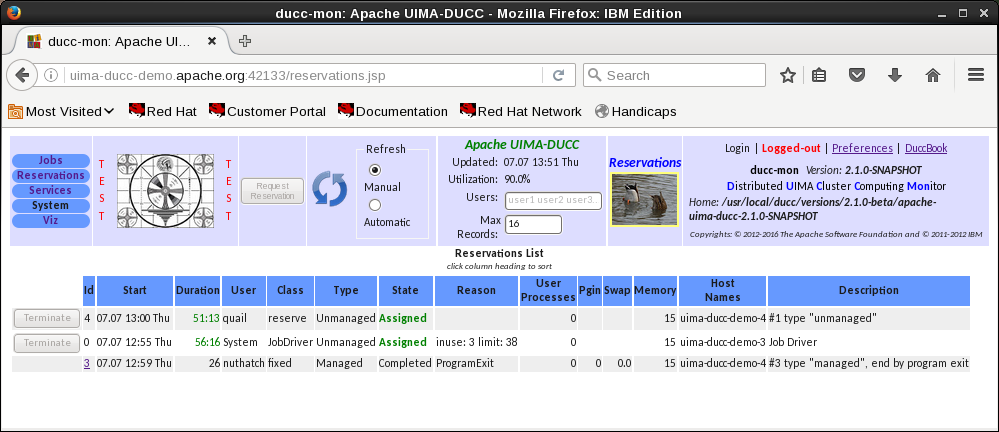
\includegraphics[width=90mm]{images/ducc-webserver/Reservations.png}
    \caption{Reservations Page}
    \end{figure}


      % Create well-known link to this spot for HTML version
      \ifpdf
      \else
      \HCode{<a name='DUCC_WS_RESERVATIONS_DETAILS'></a>}
      \fi
      % 
% Licensed to the Apache Software Foundation (ASF) under one
% or more contributor license agreements.  See the NOTICE file
% distributed with this work for additional information
% regarding copyright ownership.  The ASF licenses this file
% to you under the Apache License, Version 2.0 (the
% "License"); you may not use this file except in compliance
% with the License.  You may obtain a copy of the License at
% 
%   http://www.apache.org/licenses/LICENSE-2.0
% 
% Unless required by applicable law or agreed to in writing,
% software distributed under the License is distributed on an
% "AS IS" BASIS, WITHOUT WARRANTIES OR CONDITIONS OF ANY
% KIND, either express or implied.  See the License for the
% specific language governing permissions and limitations
% under the License.
% 
\section{Managed Reservation Details Page}
\label{sec:ws-managed-reservation-details}

This page shows details of the processes which run in a managed reservation.  The
information is divided between three tabs:

   \begin{description}
       \item[Processes] This tab contains details on all the processes contained in the
         reserved space.
       \item[Specification] This tab shows the specification for the process.
       \item[Files] This tab shows the files in the log directory.
   \end{description}  

   \subsection{Processes}
   \label{sec:ws-manres-processes}

   The processes page contains the following columns:
   \begin{description}
      \item[Id] \hfill \\
        This is the {\DUCC}-assigned numeric id of the process.  This format of this
        id is two numbers:
\begin{verbatim}
    RESID.SHAREID
\end{verbatim}
        Here, the {\em RESID} is the reservation ID.  The {\em SHAREID} is the 
        share ID assigned by the Resource Manager.  Together these form a unique
        ID for each process that runs in the reservation.
        
        Note: The current version of {\DUCC} supports only one process per managed
        reservation.  Future versions are expected to support multiple processes
        within a single managed reservation.
        
      \item[Log] \hfill \\
        This is the log name for the process. It is hyperlinked to the log itself.
        
      \item[Log Size] \hfill \\
        This is the size of the log in MB. If you find you have trouble viewing the log
        from the web server it could be because it is too big to view in the browser.
        
      \item[Host Name] \hfill \\
        This is the name of the host where the process is running (or ran).
        
      \item[PID] \hfill \\
        This is the Unix process ID (PID) of the process.
        
      \item[State Scheduler] \hfill \\
        This shows the Resource Manager state of the job. It is one of:
        
        \begin{description}
            \item[Allocated] - The resource manager has allocated resources for this process on the host.
            \item[Deallocated] - The resource manager has deallocated resources for this process on the host.
        \end{description}
        
      \item[Reason Scheduler or Extraordinary Status] \hfill \\
        These are the same as for the \hyperref[itm:job-details-sched]{job details.}

      \item[State Agent] \hfill \\
        These are the same as for the \hyperref[itm:job-details-state]{job details.}

      \item[Reason Agent] \hfill \\
        These are the same as for the \hyperref[itm:job-details-agent]{job details.}

      \item[Exit] \hfill \\
        The process exit code or signal.

      \item[Time Run] \hfill \\
        The current duration of the reservation, or total duration if it has 
        terminated.
      
      \item[PgIn] \hfill \\
        This is the number of page-in events on behalf of the process.

      \item[Swap] \hfill \\
        This is the amount of swap space on the machine being consumed by the process.
      
      \item[\%CPU] \hfill \\
        Current CPU percent consumed by the process.  This will be $>$ 100\% on 
        multi-core systems if more than one core is being used.  Each core contributes
        up to 100\% CPU, so, for example, on a 16-core machine, this can be as high
        as 1600\%.
      
      \item[RSS] \hfill \\
        The amount of real memory being consumed by the process (Resident Storage Size)

   \end{description}

   \subsection{Specification}
   \label{sec:ws-service-specification}
   This tab shows the full managed reservation specification in the form of a Java Properties
   file.  This will include all the parameters specified by the user, plus those
   filled in by {\DUCC}.
        
   \subsection{Files}
   This tab shows the files in the log directory.
        

      % Create well-known link to this spot for HTML version
      \ifpdf
      \else
      \HCode{<a name='DUCC_WS_SERVICES'></a>}
      \fi
      
    \section{Services Page}
    \label{ws:services-page}
        This page shows details of all services.           

        The Services page contains the following columns: 
        \begin{description}

            \item[Id] \hfill \\
              This is the unique numeric DUCC id of the service.  This ID is hyperlinked to a
              \hyperref[sec:ws-service-details]{Servic Details} page with extended
              details on the service.  Note that for some types of services, DUCC may not
              know more about the service than is shown on the main page.

            \item[Name] \hfill \\
              This is the unique service endpoint of the service.  
              
            \item[Type] \hfill \\
              This is the service type.
              
              There are a number of variants on service types, as discussed in the
              \hyperref[sec:services.types]{services} section of this book.  The webserver
              simplifies these into the following three values:
              \begin{itemize}
                \item Registered
                \item Submitted
                \item Implicit
              \end{itemize}
              
            \item[State] \hfill \\
              This is the state of the service with respect to the service manager.  It is a
              consolidated state over all the service instances.  Valid states are
              \begin{description}
                \item[Available] At least one service instance is responding to the service
                  pinger, indicating it is functional.
                \item[Initializing] No service instances are running but at least one instance
                  is in its UIMA-AS {\em initializing} phase.
                \item[Waiting] At least one service instance is in Running state, and the Service
                  Manager is waiting for a response from the service pinger.
                \item[NotAvailable] No service instance is running. 
                \item[Stopping] The service has been stopped for some reason, but not all 
                  instances have terminated.
              \end{description}

              DUCC will start dependent jobs ONLY if it's services are in state Available.  Otherwise
              DUCC attempts to start the service, and if successful, allows the job to start.  

              If a job is already running and a service becomes other than Available, the
              \hyperref[sec:ws.jobs-page]{jobs page} indicates the service is not available but the job is 
              allowed to continue.
              
            \item[Pinger] \hfill \\
              This indicates whether the Service Manager is running a pinger for the service.
              
            \item[Health] \hfill \\
              {\em Health} is a status returned by each pinger and is the result of that pinger's
              evaluation of the state of the service.  It is shown as on of
              \begin{itemize}
                \item {\em Good}
                \item {\em Bad}
              \end{itemize}
              Both terms are highly subjective.  Pingers may return a summary of the underlying
              data used to label a service as good or bad.  That status is shown as a hover over
              this field.
              
            \item[Instances] \hfill \\
              This is the number of instances (processes) currently registered for the service.  

            \item[Deployments] \hfill \\
              This is the number of actual instances deployed for the service.  Note that this may
              be greater, or less, than the number of registered instances, if the service owner
              decides to temporarily start or stop additional instances.

            \item[User] \hfill \\
              This is the userid of the service owner.
              
            \item[Class] \hfill \\
              This is the scheduling class the service is running in. 
              
              If a service is registered as ``ping-only'', no resources are allocated for it.  This
              is shown as a class of {\tt ping-only}.
              
            \item[Size] \hfill \\
              This is the memory size, in GB, of each service instance

            \item[Jobs] \hfill \\
              This is the number of jobs currently using the service.  The IDs of the jobs are
              shown as hovers over this field.

            \item[Services] \hfill \\
              Services may themselves depend on other services.  This field shows the number of
              services dependent on this service.  The dependent service IDs are shown with a 
              hover over the field.

            \item[Reservations] \hfill \\
              This field shows the number of
              managed reservations dependent on this service. The IDs of the managed reservations
              rea shown as a hover over the field.

              
            \item[Description] \hfill \\
              This is the description string from the --description string from submit.
        \end{description}


      % Create well-known link to this spot for HTML version
      \ifpdf
      \else
      \HCode{<a name='DUCC_WS_SERVICE_DETAILS'></a>}
      \fi
      % 
% Licensed to the Apache Software Foundation (ASF) under one
% or more contributor license agreements.  See the NOTICE file
% distributed with this work for additional information
% regarding copyright ownership.  The ASF licenses this file
% to you under the Apache License, Version 2.0 (the
% "License"); you may not use this file except in compliance
% with the License.  You may obtain a copy of the License at
% 
%   http://www.apache.org/licenses/LICENSE-2.0
% 
% Unless required by applicable law or agreed to in writing,
% software distributed under the License is distributed on an
% "AS IS" BASIS, WITHOUT WARRANTIES OR CONDITIONS OF ANY
% KIND, either express or implied.  See the License for the
% specific language governing permissions and limitations
% under the License.
% 
\section{Service Details Page}
\label{sec:ws-service-details}

This page shows details of the processes which implement. 

The information is divided between four tabs:

   \begin{description}
       \item[Deployments] This tab contains details on all the processes implementing
         the service, if any.
       \item[Registry] This tab shows the registration information for the service.
       \item[Files] This tab shows the files in the log directory. 
       \item[History] This tab contains details on all the completed processes implementing the service, if any.  
   \end{description}  

   \subsection{Deployments}
   \label{sec:ws-services-processes}

   The deployments page contains the following columns:
   \begin{description}
      \item[Id] \hfill \\
        This is the {\DUCC}-assigned numeric id of the process.  This format of this
        id is two numbers:
\begin{verbatim}
    RESID.SHAREID
\end{verbatim}
        Here, the {\em RESID} is the Orchestrator assigned instance ID.  The {\em SHAREID} is the 
        instance ID assigned by the Resource Manager.  Together these form a unique
        ID for each process that runs in the service.
               
      \item[State] \hfill \\
        The state of this service instance.
               
      \item[Services] \hfill \\
        The current state of service dependencies.
                                
      \item[Log] \hfill \\
        This is the log name for the process. It is hyperlinked to the log itself.
        
      \item[Log Size] \hfill \\
        This is the size of the log in MB. If you find you have trouble viewing the log
        from the web server it could be because it is too big to view in the browser.
        
      \item[Host Name] \hfill \\
        This is the name of the node where the process is running (or ran).
        
      \item[PID] \hfill \\
        This is the Unix process ID (PID) of the process.
       
      \item[Memory] \hfill \\
        The service process actual memory size (GB).
                
      \item[State Scheduler] \hfill \\
        This shows the Resource Manager state of the service instance. It is one of:
        
        \begin{description}
            \item[Allocated] - The node is still allocated for this service instance by the RM.
            \item[Deallocated] - The resource manager has deallocated the resources for the service instance on
              this node.
        \end{description}
        
      \item[Reason Scheduler or Extraordinary Status] \hfill \\
        These are the same as for the \hyperref[itm:job-details-sched]{job details.}

      \item[State Agent] \hfill \\
        These are the same as for the \hyperref[itm:job-details-state]{job details.}

      \item[Reason Agent] \hfill \\
        These are the same as for the \hyperref[itm:job-details-agent]{job details.}

      \item[Exit] \hfill \\
        The process exit code or signal.

      \item[Time Init] \hfill \\
        Most services are UIMA-AS services and therefore have an {\em initialization} phase
        to their lifetimes.  This field shows the time spent in that phase.

      \item[Time Run] \hfill \\
        The current duration of the instance, or total duration if it has 
        terminated.
        
      \item[Time GC] \hfill \\
        This is amount of time spent in Java Garbage Collection for the process.

      \item[Pgin] \hfill \\
        This is the number of page-in events on behalf of the process.
        
      \item[Swap] \hfill \\
        This is the amount of swap space on the machine being consumed by the process.
        
      \item[\%CPU] \hfill \\
        Current CPU percent consumed by the process.  This will be $>$ 100\% on 
        multi-core systems if more than one core is being used.  Each core contributes
        up to 100\% CPU, so, for example, on a 16-core machine, this can be as high
        as 1600\%.

      \item[RSS] \hfill \\
        The amount of real memory being consumed by the process (Resident Storage Size)

      \item[JConsole URL] \hfill \\
        This is a URL that can be used to connect via JMX to the processes, e.g. via
        jconsole.

   \end{description}

   \subsection{Registry}
   \label{sec:ws-managed-reservation-specification}
   This tab shows the full service specification in the form of a Java Properties
   file.  This will include all the parameters specified by the user, plus those
   filled in by {\DUCC}.
        
   The registry for a Service contains two types of entries:
   \begin{enumerate}
     \item Service specification properties, prefixed with ``svc''. These comprise
       the service specification that the Service Manager submits on behalf of
       a user in order to start registered services.
     \item Meta properties, prefixed with ``meta''.  This is the Service Manager's state
       record for the service as it is running.  In addition to state it contains
       properties required for service registration that are not used for
       service submission.
   \end{enumerate}
           
   \subsection{Files}
   This tab shows the files in the log directory.
   
           
   \subsection{History}
   This tab shows the completed service instances.
   


      % Create well-known link to this spot for HTML version
      \ifpdf
      \else
      \HCode{<a name='DUCC_WS_SYSTEM'></a>}
      \fi
      % 
% Licensed to the Apache Software Foundation (ASF) under one
% or more contributor license agreements.  See the NOTICE file
% distributed with this work for additional information
% regarding copyright ownership.  The ASF licenses this file
% to you under the Apache License, Version 2.0 (the
% "License"); you may not use this file except in compliance
% with the License.  You may obtain a copy of the License at
% 
%   http://www.apache.org/licenses/LICENSE-2.0
% 
% Unless required by applicable law or agreed to in writing,
% software distributed under the License is distributed on an
% "AS IS" BASIS, WITHOUT WARRANTIES OR CONDITIONS OF ANY
% KIND, either express or implied.  See the License for the
% specific language governing permissions and limitations
% under the License.
% 

\section{System Pages}
\label{sec:system-details}

These pages show information relating to the {\DUCC} System itself:
\begin{description}
  \item[Administration]This displays system administrators and implements
    the interface to various administrative controls.
  \item[Broker] This shows selective information for the system's broker.
  \item[Classes] This shows the system's scheduling class definitions.
  \item[Daemons] This shows the status of all {\DUCC} processes.
  \item[DuccBook] This is a link to the book you are reading.
  \item[Machines] This shows details of all the machines (nodes) in the {\DUCC} cluster.
\end{description}

\subsection{Administration}

   This page has two tabs:
   \begin{description}   
     \item[Administrators] This shows the user-ids that are authorized to administer
       {\DUCC}.  In addition to executing the ``Control'' functions described below,
       administrators may cancel any job, reservation, or service, and may modify
       services they do not own.  

       In order to perform administrative functions, the following must be satisfied:
       \begin{enumerate}
         \item The user is logged-in to the web server.
         \item The user is a registered administrator.
         \item The user has set the role as ``administrator'' in the {\DUCC} Preferences
           page.  This is a safeguard so that administrators who are also users
           are less likely to inadvertently affect other people's jobs.
       \end{enumerate}
     \item[Control] Currently {\DUCC} supports a single administrative control function
       via the web server: Stop new job submissions and re-enable them.  If submissions
       are blocked, all existing work runs normally, but no new work is accepted.
     \end{description}


\subsection{Broker}
This page shows selective information for the system's broker.
Information includes host, port, version, uptime, memory used, threads, load average, topics and queues.

\subsection{Classes}
This page shows the definitions of the {\DUCC} scheduling classes.  The scheduling classes are
discussed in more detail in the \hyperref[sec:rm.job-classes]{Resource Manager} section.

\subsection{Daemons}
\label{sec:system-details.daemons}

This page shows the current state of all {\DUCC} processes.  By default, only the administrative
processes, Broker, Database, Orchestrator, ProcessManager, ResourceManager, ServiceManager, and Webserver are
shown.  A button in the upper left of the page titled ``Show Agents'' enables display of
the status of all the {\DUCC} agents as well. (Agents are suppressed by default because the
page is expensive to render for large systems.)

The columns shown on this page include

   \begin{description}
      \item[Status] \hfill \\
        This indicates whether the daemon is running and broadcasting state {\em up},
        or not {\em down}.  
        
        All {\DUCC} daemons broadcast a heartbeat containing process state.  If the Status
        is {\em down}, either the daemon is not functioning, or something is preventing
        state from reaching the web server via {\DUCC}'s ActiveMQ instance.

      \item[Daemon Name] \hfill \\
        This is the name of the process.

      \item[Boot Time] \hfill \\ 
        This shows the date and time of the latest boot of the specific process.
          
      \item[Host IP] \hfill \\ 
        This is the IP address of the processor where the process is running.

      \item[Host Name] \hfill \\ 
        This shows the hostname of the processor where the process is running.

      \item[PID] \hfill \\ 
        This is the Unix process Id of the {\DUCC} process.

      \item[Publication Size (last)] \hfill \\ 
        This shows the size of the most recent state publication of the process, in bytes.

      \item[Publication Size (max)] \hfill \\ 
        This shows the size of the largest state publication of the process, in bytes.

      \item[Heartbeat (last)] \hfill \\ 
        This shows the number of seconds since the last state publication for the process. 
         Large numbers here indicate potential cluster or {\DUCC} problems.

      \item[Heartbeat (max)] \hfill \\ 
        This shows the longest delay since a state publication for the process was received
        at the web server.  Large numbers here indicate potential cluster or {\DUCC} problems.

      \item[Heartbeat (max) TOD] \hfill \\ 
        This shows the time the longest delay of a state publication occurred.

      \item[JConsole URL] \hfill \\ 
        This is the jconsole URL for the process.

   \end{description}
      
\subsection{Machines}

This page shows the states of all the machines (nodes) in the {\DUCC} cluster.

The columns shown on this page include

   \begin{description}
      \item[Status] \hfill \\
        This shows the current state of a machine.  Values include:
        \begin{description}
          \item[defined] The node is in the {\DUCC}
            \hyperref[sec:admin-ducc.nodes]{nodes file}, but no {\DUCC} process has been
            started there, or else there is a communication problem and
            the state messages are not being delivered.
            \item[up] The node has a {\DUCC} Agent process running on it and the
              resource manager is receiving regular heartbeat packets from it.
            \item[down] The node had a healthy {\DUCC} Agent on it at some point
              in the past (since the last {\DUCC} boot), but the resource manager
              has stopped receiving heartbeats from it. 

              The agent may have been manually shut down, may have crashed, or there
              may be a communication problem.

              Additionally, very heavy loads from jobs running the the node can cause
              the {\DUCC} Agents heartbeats to be delayed.
        \end{description}

      \item[IP] \hfill \\
        This is the IP address of the node.


      \item[Name] \hfill \\
        This is the hostname of the node.

      \item[Nodepool] \hfill \\
        This is the host nodepool.

      \item[Memory(GB) usable] \hfill \\
        This is the amount of usable memory, in GB, as reported by each machine.  
        This is the maximum amount that can be allocated by the resource manager.
        
        Usually the amount will be slightly less than the installed memory.  This is because
        a small bit of memory is usually reserved by the hardware for its own purposes.  For 
        example, a machine with 48GB of installed memory may report only 47GB available.

      \item[Memory(GB) free] \hfill \\
        This is the amount of free memory, in GB, as reported by each machine.
        This is the amount not presently allocated by the resource manager.
        
      \item[CPU] \hfill \\
        This is the host CPU one minute load average.
        
      \item[Swap(GB) inuse] \hfill \\
        This is the total size in-use swap data.  {\DUCC} shows any value greater than 0 in
        red as swapping can very significantly slow applications.  However, swap use does
        not always mean there is a performance problem.  This is flagged by {\DUCC} simply
        as an alert of a potential problem

      \item[Swap(GB) free] \hfill \\
        This is the total size of swap area.  

      \item[C-Groups] \hfill \\
        If on then C-Groups are in use and processes deployed by {\DUCC} will
        be limited in resource consumption.


      \item[Alien PIDs] \hfill \\
        This shows the number of processes not owned by {\DUCC}, the operating system, or
        jobs scheduled on each node.  The Unix Process IDS of these processes is displayed
        in a hover.

        {\DUCC} preconfigures many of the standard operating 
        \hyperref[itm:props-rogue.process]{system process} and 
        \hyperref[itm:props-rogue.user]{userids}.  This list may be updated by each
        installation.

        A common cause of alien PIDs is errant process run in unmanaged reservations.  A
        user may reserve a machine for use as a sandbox.  If the reservation is released
        without properly terminating all the processes, they may linger.  When {\DUCC} 
        schedules the node for other purposes, significant performance penalties may be
        paid due to competition between the legitimately scheduled work and the leftover
        ``alien'' processes.  The purpose of this column is to bring attention to this situation.


      \item[Heartbeat(last)] \hfill \\
        This shows the number of seconds since the last agent heartbeat from this machine.

      \end{description}
      


      % Create well-known link to this spot for HTML version
      \ifpdf
      \else
      \HCode{<a name='DUCC_WS_Viz'></a>}
      \fi
      % 
% Licensed to the Apache Software Foundation (ASF) under one
% or more contributor license agreements.  See the NOTICE file
% distributed with this work for additional information
% regarding copyright ownership.  The ASF licenses this file
% to you under the Apache License, Version 2.0 (the
% "License"); you may not use this file except in compliance
% with the License.  You may obtain a copy of the License at
% 
%   http://www.apache.org/licenses/LICENSE-2.0
% 
% Unless required by applicable law or agreed to in writing,
% software distributed under the License is distributed on an
% "AS IS" BASIS, WITHOUT WARRANTIES OR CONDITIONS OF ANY
% KIND, either express or implied.  See the License for the
% specific language governing permissions and limitations
% under the License.
% 

    \section{Visualization}
    \label{sec:ws.vizualization}
       This page shows a visualization of all scheduled work.  Every host is represented by a square
       whose area is proportional to the amount of memory on the host.  If work is scheduled to a
       host, it is represented by a rectangle whose area is proportional to the amount of memory
       that is scheduled for the work.  In a multi-user environment, each userid is mapped into 
       a different color, making it possible to see the usage per-user.

       Hovers are provided to show the real memory size of each host, the schedulable memory for
       each host, and the amount of memory scheduled for each bit of work.

       If multiple allocations are made on a single host for the same job or service, the rectangles
       are combined into a single rectangle, reducing clutter and better showing the actual usage
       of the job (or service).   

       Clicking on any box representing scheduled work sends the browser to the details page for 
       the corresponding work.

       The screenshot below shows a visualization with a handful of 127GB hosts, 48GB hosts, and
       32GB hosts.  Regular UIMA-AS jobs show as untextured boxes; for example, job 6080, owned
       by user Hilaria, running in a 37GB allocation in host bluej291-41 which is a 127GB host.

       Hosts bluej291-45 and 291-46 are running Managed Reservations, which are shown with
       crosshatches from lower-left to upper right.

       Hosts bluej291-37 and bluej291-40 are running Unmanaged Reservations, shown with
       vertical-horizontal crosshatches.

       Below bluej291-34, bluej291-36, bluej293-49, and bluej293-60 are running {\DUCC}-managed
       services, shown by crosshatching from upper-left to lower-right.

       The host representations may be sorted by clicking on the ``size'' or the ``name'' text
       near the top of the display.


           \begin{figure}[ht!]
    \centering
    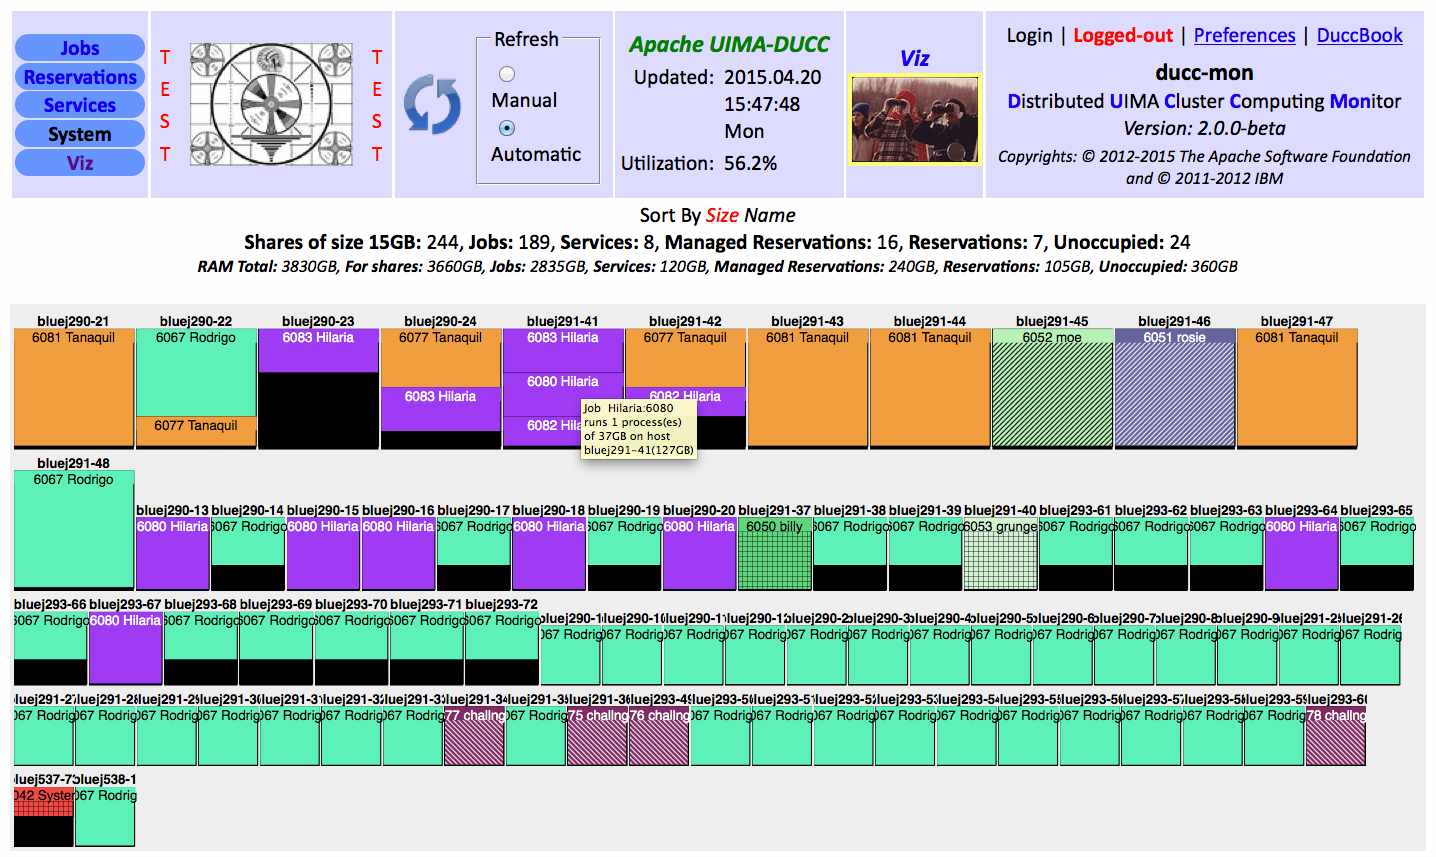
\includegraphics[width=160mm]{images/ducc-webserver/viz.jpg}
    \caption{Visualization}
    \end{figure}


